\documentclass[12pt]{kiarticle} 
\graphicspath{{pictures/}}
\DeclareGraphicsExtensions{.pdf,.png,.jpg,.eps}
\usepackage{indentfirst}
\newcommand{\del}{\ensuremath{\delta}}
\newcommand{\co}{\ensuremath{\mathrm{const}}}
\newcommand{\D}{\ensuremath{\mathcal{D}}}
%%%
\fancyhead[L]{Вопрос по выбору --- термодинамика, 2017\hfil}
\fancyhead[R]{\hfil Иванов Кирилл, 625 группа }



\begin{document}

\begin{titlepage}
	\begin{center}
		\large 	Московский физико-технический университет \\
		Факультет общей и прикладной физики \\
		\vspace{0.2cm}
		
		\vspace{4.5cm}
		Вопрос по выбору во 2 семестре \\ \vspace{0.2cm}
		\large (Общая физика: термодинамика) \\ \vspace{0.2cm}
		\LARGE \textbf{Энтропия. Второе начало термодинамики}
	\end{center}
	\vspace{2.3cm} \large
	
	\begin{center}
		Автор: \\
		Иванов Кирилл,
		625 группа
		\vspace{10mm}
		
		Семинарист: 
		
		Слободянин Валерий Павлович
		
		
	\end{center}
	
	\begin{center} \vspace{50mm}
		г. Долгопрудный \\
		 2017 год
	\end{center}
\end{titlepage}

%%%%%%%%%%
%%%%%%%%%%
%%%%%%%%%%%%%%%%%%%%%%%%%%%%%%%%%%%

\section{Введение}

В курсе термодинамики, изучаемом в МФТИ, постулируют сначала так называемое "<нулевое"> и затем первое начала термодинамики, а затем, изучая тепловые машины и циклы, приходят ко второму началу термодинамики. В процессе такого перехода весьма естественно формируется определение \textbf{энтропии} как приведённого тепла: 

\begin{equation}\label{entmipt}
 dS = \dfrac{\del Q}{T}
\end{equation}

Впоследствии с помощью этого получается обобщение первого начала термодинамики в виде $ TdS = dU + \del A $ и энтропии как одной изи четырех термодинамических потенциалов. 

Мы же попробуем ввести понятие энтропии немного по-другому, опираясь на другие понятия.

\section{Вывод энтропии}

\subsection{Определение условных параметров} \label{ifTS}

Рассмотрим произвольный сосуд с некоторым газом. Весьма естественно определить такие макропараметры, как \textit{давление} $ P $ и \textit{объем} $ V $ из чисто логических и механических соображений. Введём также понятие \textit{условной температуры} $ \tau $ как некого третьего параметра нашей системы и будем считать его "<мерой нагретости тела"> (понимая, однако, наличие и более объективного смысла температуры, на котором мы не будем останавливаться в данной работе). 

 \begin{wrapfigure}{l}{0.35\linewidth} 
	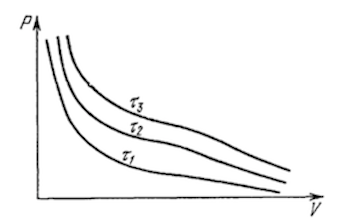
\includegraphics{tempdef}
	\caption{Семейство изотерм с температурой $ \tau_i $}
\end{wrapfigure}

Определив \textit{термостат} как тело с бесконечно большой теплоёмкостью, поместим туда наш газ. Зафиксировав в термостате этот параметр, будем изменять $ P $ и $ V $, и так сделаем для разных температур. Опыты показывают, что для каждой температуры можно построить кривую (\textit{изотерму}) на плоскости $ PV $, которые не будут пересекаться, и при нормальных условиях будут приближённо иметь вид гипербол. 

Тогда такой газ мы назовём \textit{идеальным}, а условная температура $ \tau = \tau (P, V) $ будет являться функцией состояния системы. Кроме того, для уравнения состояния будет справедливо следующее:

\begin{equation}\label{defte}
PV = \co \te \tau (P, V) = \tau (PV)
\end{equation}

Так можно сформулировать \textbf{принцип температуры} о существовании функции состояния, остающейся неизменной при любом процессе на изотерме (в термостате).

\begin{wrapfigure}{l}{0.34\linewidth} 
	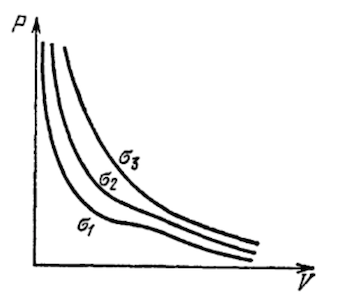
\includegraphics{entdef}
	\caption{Семейство адиабат с энтропией $ \sigma_i $}
\end{wrapfigure}

Теперь определим \textit{адиабат} как абсолютно теплонепроницаемое тело и получим другое семейство кривых с параметром \textit{условной энтропии}. Так как они не пересекаются, то $ \sigma = \sigma (P, V) $ тоже однозначная функция состояния системы, и можно сформулировать \textbf{принцип энтропии}. Для введенного выше идеального газа  уравнение состояния имеет вид (полученный опытным путем)

\begin{equation}\label{defent}
PV^\gamma = \co \te \sigma (P, V) = \sigma (PV^\gamma)
\end{equation}

где $ \gamma > 1 $ --- \textit{показатель адиабаты}. Таким образом, обозначив константы из \eqref{defte} и \eqref{defent} за $ x, y $ соответственно, мы получаем однозначное решение этой системы в виде

\begin{equation}\label{xy}
P = \left( \dfrac{x^\gamma}{y} \right)^\frac{1}{\gamma -1}, \quad V = \left (\dfrac{y}{x} \right )^\frac{1}{\gamma -1} 
\end{equation}

\subsection{Абсолютные параметры}

Результаты, полученные в \eqref{xy}, также показывают нам очень важное свойство --- каждая адиабата и каждая изотерма пересекаются в одной и только одной точке плоскости $ PV $. Тогда мы получаем, что соотношение между парами параметров газа $ P, V $ и $ \tau, \sigma $ является \textbf{взаимно однозначным}, и плоскость $ PV $  эквивалентна $ \tau \sigma $-плоскости. Рассмотрим это поподробнее.

Переход одной плоскости в другую эквивалентен следующему переходу элементарных площадей: 

\begin{equation}\label{D}
dP dV \st \D d\tau d\sigma
\end{equation}

где $ \D  = \pdd{(P, V)}{(\tau, \sigma)} $ --- \textit{якобиан}. Тогда естественно положить $ \D = 1 $ для полного равноправия наших плоскостей. Эта нормировка позволяет выбрать определённые температурные и энтропийные шкалы, и отсчитываемые по ним величины мы будем называть уже \textit{абсолютными} температурой $ T $ и энтропией $ S $. Пользуясь вышевведенными обозначениями и считая $ T = T(x), S = S(y) $, мы воспользуемся формулой произведения якобианов: $  \pdd{(P, V)}{(\tau, \sigma)} = 1 \ekv  \pdd{(T, S)}{(x, y)} \pdd{(x, y)}{(P, V)} = 1 \te$

\begin{equation}\label{DD}
\begin{vmatrix}
\pdd{T}{x} & \pdd{T}{y} \\
\pdd{S}{x} & \pdd{S}{y} \\
\end{vmatrix} 
\x
\begin{vmatrix}
\pdd{x}{P} & \pdd{x}{V} \\
\pdd{y}{p} & \pdd{y}{V} \\
\end{vmatrix}
=
\left( \dfrac{dT}{dx} \dfrac{dS}{dy} - 0\right) \left( V\x \gamma PV^{\gamma - 1} - P\x V^\gamma\right) = T' S' y(\gamma - 1) = 1
\end{equation}

Так мы получаем следующее соотношение, в котором левая часть является функцией от $ x $, а правая от $ y $:

\begin{equation}\label{T'S'}
T' = \dfrac{1}{S'y(\gamma - 1)}
\end{equation}

Тогда эти части равны одной и той же константе, которую мы обозначим за $ \frac{1}{R} $:

\begin{equation}\label{R}
T' = \dfrac{dT}{dx} = \dfrac{1}{R}, \quad S' = \dfrac{dS}{dy} = \dfrac{R}{\gamma - 1} \dfrac{1}{y}
\end{equation}

Проинтегрируем эти уравнения:
\begin{equation}\label{TS}
\sys{
&T = \dfrac{x}{R} + C_T = \dfrac{PV}{R}  + C_T \\
&S = \dfrac{R}{\gamma -1} \ln y + C =  \dfrac{R}{\gamma -1} \ln PV^\gamma + C
}
\end{equation} 

Где, конечно, $ C_T, C $ --- константы интегрирования. Для удобства превратим величину под логарифмом в безразмерную, выбрав $ C = S_0 - \frac{R}{\gamma -1} \ln P_0V^\gamma_0$:

\begin{equation}\label{S}
S - S_0 = \dfrac{R}{\gamma -1} \ln  \dfrac{PV^\gamma}{P_0V_0^\gamma} = \dfrac{R}{\gamma -1} \ln \dfrac{(T - C_T) V^{\gamma - 1}}{(T_0 - C_T) V^{\gamma -1 }_0} = \dfrac{R}{\gamma -1} \ln \frac{(T - C_T)^\gamma P^{1 - \gamma}}{(T_0 - C_T)^\gamma P_0^{1 -\gamma}}
\end{equation}

Так мы получили соотношения для температуры и энтропии, опираясь на введенные в параграфе \ref{ifTS} утверждения. Постоянная $ R $ будет определять лишь масштаб наших шкал, и выбрав ее равной $ R = 8,31 $ Дж/К$ \x $моль, получим шкалу Кельвина для температуры. Используя подобные рассуждения, мы можем ввести адиабатический и изотермические потенциалы через работу с якобианами, и пользуясь законом сохранения энергии в виде первого начала термодинамики, мы можем получить и соотношение $ \del Q = TdS $, что позволит доказать классические  равенства $ C_T = 0 $ и  $ \gamma = \frac{C_P}{C_V}  $.

\subsection{Плоскость TS}

\begin{wrapfigure}{l}{0.45\linewidth} 
	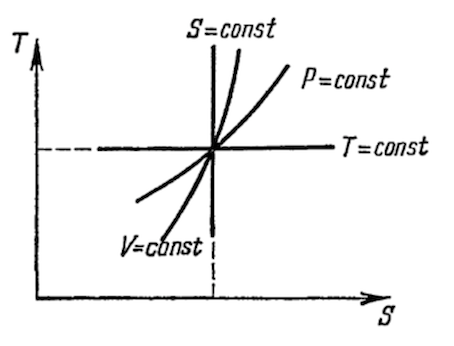
\includegraphics{TS}
	\caption{Изопроцессы на плоскости $ TS $}
	\label{GrafTS}
\end{wrapfigure}

Пользуясь первым уравнением из \eqref{TS} и первым равенством из \eqref{S}, мы получаем систему:

\begin{equation}\label{sysTS}
\sys{
&PV = RT \\
&PV^\gamma = \co \; e^{(\gamma - 1)\frac{S}{R}}
}
\end{equation}

Тогда, выражая из первого давление для изохорного и объем для изобарного процессов, второе уравнение будет иметь следующий вид:

\begin{equation}\label{}
\sys{
& V = \co \te T = T_1(V) \; e^{(\gamma - 1)\frac{S}{R}} \\
& P = \co \te T = T_2(P) \; e^{(\gamma - 1)\frac{S}{\gamma R}} \\
}
\end{equation}

Где $ T_1(V), T_2(P) $ --- функции от объема и давления, равные константам при фиксированных аргументах. Это и позволяет нам получить график всех знакомых изопроцессов на рис.\ref{GrafTS}. 


%\section*{Список литературы}
%
%\begin{enumerate}
%	
%	\item 
%	
%\end{enumerate}














\end{document}
	
